\documentclass[10pt,a4paper, twoside]{report}
\usepackage[utf8]{inputenc}  
\usepackage[T1]{fontenc}      
\usepackage[francais]{babel}
\usepackage{amsmath}
\usepackage{amsfonts}
\usepackage{amssymb}
\usepackage{graphicx}
\usepackage{hyperref}
\usepackage{caption}
\usepackage{eurosym}
\usepackage{wrapfig}
\usepackage{rotating}
\usepackage{array, multirow}
\usepackage[usenames,dvipsnames,svgnames,table]{xcolor}
\newcolumntype{M}[1]{>{\centering\arraybackslash}m{#1}}
\renewcommand{\baselinestretch}{1.5}
\newcommand{\mychapter}[2]{
	\setcounter{chapter}{#1}
	\setcounter{section}{0}
	\chapter*{#2}
	\addcontentsline{toc}{chapter}{#2}
}

\author{Thomas Citharel}
\title{Rapport de stage}
\begin{document}
	\maketitle
	\newpage\null\thispagestyle{empty}\newpage
	\mychapter{0}{Remerciements}
	Merci maman merci papa
	\setcounter{tocdepth}{1}
	\begingroup\makeatletter
	\def\@makeschapterhead#1{%
		{\parindent \z@ \raggedright
			\normalfont
			\interlinepenalty\@M
			\Huge \bfseries  #1\par\nobreak
		}}\makeatother
		\tableofcontents
		\endgroup
	
	\mychapter{1}{Introduction}
	Dans le cadre des études que j'effectue à l'\textbf{IUT d'Orléans} dans le but d'obtenir un Diplôme Universitaire de Technologie, je devais effectuer un stage d'une durée de 10 semaines afin de valider ce diplôme. Ce stage a pour but d'acquérir une première expérience professionnelle en validant les connaissances apprises durant l'année et en exerçant des compétences au travers de la réalisation d'un projet.
	\\
	
	Ce stage s'est pour ma part effectué du 20 juin au 26 août 2016 au sein de l'association \textbf{Framasoft} dont les buts sont la promotion, la diffusion et le développement de logiciels libres, de services libres en ligne et de la culture libre.
	\\
	
	J'avais pour but de développer et mettre en place une alternative à Google Calendar nommée \textbf{Framagenda}. En accord avec mon maître de stage, le choix de quelle application existante prendre pour base parmi plusieurs applications existantes s'est porté sur le logiciel libre ownCloud dont la fonctionnalité principale est le service de stockage et de sauvegarde de fichiers mais qui propose de nombreuses applications tierces dont une faisant office de calendrier.
	
	\chapter{Les acteurs du stage}
	\section{IUT}
	L'\textbf{Institut Universitaire de Technologie d'Orléans - La Source} fait partie intégrante de l'Université d'Orléans - Tours. Il est composé de différents départements dont celui d'Informatique. Les domaines enseignés sont théoriques comme pratiques, et des enseignements complémentaires dont une langue vivante et des cours de Gestion et de communication professionnelle y sont également donnés.
	
	\begin{figure}[ht]
		\centering
		
\includegraphics[width=0.35\textwidth]{images/logo-iut.png}
		\caption*{Logo de l'IUT et de l'Université d'Orléans}
		\label{normal_case}
	\end{figure}
	
	La formation conduisant à un Diplôme Universitaire de Technologie est d'ordinaire effectuée sur la période de deux années mais l'IUT offre également aux étudiants ayant déjà un parcours dans l'enseignement supérieur la possibilité d'effectuer cette formation en une année.
	
	La formation se conclut par un stage obligatoire pour mettre en application les connaissances acquises au fil de l'année, exercer ses compétences en participant à un projet non-scolaire et en acquérir de nouvelles.
	
	\section{Framasoft}
	\subsection{Présentation de la structure d'accueil}
	
	Le site internet Framasoft (pour \textbf{fra}nçais et \textbf{ma}thématiques) a été fondé par le professeur de mathématiques Alexis KAUFMANN en 2001. Il se présente à cette époque comme un annuaire de logiciels libres et gratuits comme ressources pédagogiques pour enseignants.
	
	\begin{figure}[ht]
		\centering
		
\includegraphics[width=0.25\textwidth]{images/Framasoft-Logo.png}
		\caption*{Logo actuel de Framasoft}
		\label{normal_case}
	\end{figure}
	
	Le site Framasoft se développe en réseau avec l'intégration de tutoriels et du forum Framagora. Une association Loi 1901 éponyme est fondée en 2004 pour gérer le réseau et acquerra le statut d'association à but non lucratif quatre ans plus tard. L'annuaire se sépare des logiciels gratuits non libres la même année, et s'ouvre à d'autres systèmes d'exploitation que Windows.
	\\
	
	Framasoft s'oriente alors vers des missions de promotion du logiciel libre auprès du grand public, et veut devenir un réseau de partage de connaissances. Deux autres axes de campagnes sont également abordés à ce moment : la culture libre et les services libres. Des projets comme la \textit{Framakey}, une clé USB contenant une sélection de logiciels libres à utiliser directement sous Windows, Linux ou MacOS X sont lancés à ce moment.
	\\
	
	C'est en 2006 que Framasoft publie son premier Framabook, « Utilisez Thunderbird 1.5 ! » sous licence Creative Commons. Au départ constituée uniquement de manuels, la collection s'étoffe quelques années plus tard avec des romans et des bandes-dessinées. C'est aujourd'hui une vingtaine de Framabooks tous sous licence libre (Creative Commons, GNU FDL, Licence Art Libre, etc) qui constituent cette collection.
	
	Les actions de l'association, des tribunes et des traductions de prises de position en langue étrangères sont publiées dans le Framablog, qui compte aujourd'hui près de 2000 articles. Des partenariats avec l'Éducation Nationale aboutissent en 2009 et 2010 à la création d'un Framadvd de ressources pédagogiques.
	\\
	
	À compter de l'année 2011, Framasoft commence à sortir des services web comme Framapad (un éditeur collaboratif), Framadate (un outil pour planifier des événements via sondage) ou encore Framacalc (un tableur en ligne).
	\\
	
	À l'automne 2014 est annoncée la campagne \textbf{Dégooglisons Internet} qui a pour but de montrer au public qu'ils ne sont pas condamnés à utiliser des services qui ne respectent pas leur vie privée (plus de détails-ci dessous \ref{subsec:degoogl}).
	\\
	
	Aujourd'hui, Framasoft compte une trentaine de membres dont cinq salariés et deux stagiaires, et est une des associations francophones les plus en pointe sur le sujet des logiciels libres et du respect de la vie privée.
	\\
	
	Côté services, on compte aujourd'hui plus d'un demi-million de visites sur tous les sites du réseau chaque mois, un nouveau sondage créé environ chaque minute sur Framadate et 100 000 pads actuellement actifs sur Framapads. Il y a aujourd'hui une vingtaine de livres édités par Framasoft. Enfin, grâce à l'éclatement géographique de ses membres, Framasoft peut être présent sur une énorme partie des événements liés au logiciel libre dans le monde francophone.
	\\
	
	L'association possède un budget de l'ordre de 200 000\euro{} financés à 90\% par les dons, dont la grande majeure partie vient de particuliers. Le reste est issu de la vente de produits dérivés et de rares prestations techniques.
	\\
	
	Il est important de noter que Framasoft n'ambitionne pas de devenir le prochain géant du web. L'association reste à but non lucratif et a de plus une volonté de décentraliser ses activités au sein de structures locales qui seraient des « hébergeurs de services de proximité ».
	\\
		
	L'association ayant comme but de sensibiliser le grand public aux valeurs du logiciel libre, elle est très souvent invitée à s'exprimer lors de manifestations en rapport avec le sujet, comme celle à laquelle j'ai pu participer à Nevers le week-end du 24 au 26 Juin.
	
	\subsection{Dégooglisons Internet}
	\label{subsec:degoogl}
	
	En octobre 2014, la campagne \href{https://degooglisons-internet.org/}{\textbf{\textit{Dégooglisons} Internet}} est lancée par Framasoft afin de montrer au public que des solutions à base de logiciel libre sont possibles face aux services proposés par les \textit{géants du net} (aussi nommés \textbf{GAFAM} pour \textbf{G}oogle, \textbf{A}mazon, \textbf{F}acebook, \textbf{A}pple et \textbf{M}icrosoft, mais il y en existe une multitude d'autres).
	

	\centerline{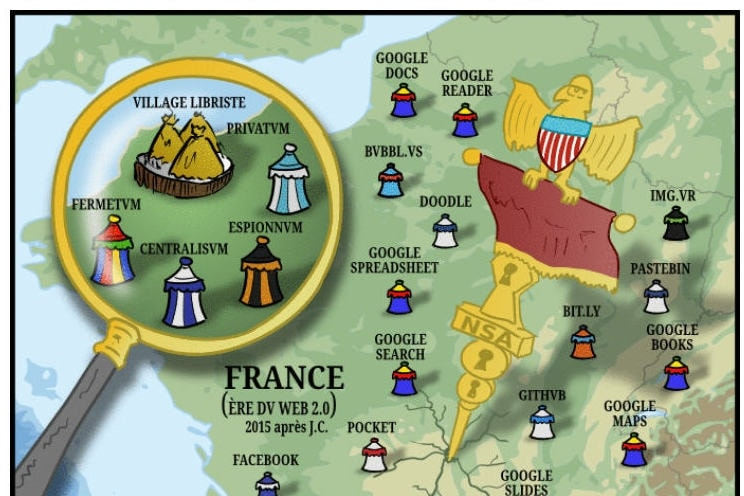
\includegraphics[width=1\textwidth]{images/degooglisons-internet.jpg}}

	
	En plus de ceux proposés avant le début de la campagne (Framapad, Framadate, ...), Framasoft a ouvert une vingtaine de services en ligne et il en est prévu davantage d'ici la fin de la campagne en 2018 (cf. Annexe \ref{sec:listeservices}).
	
	Framasoft utilise donc des applications web libres existantes ou développe ses propres alternatives pour proposer à des personnes non-techniques des services viables.
	Ainsi, l'association a fait développer des solutions spécialement pour proposer Framapic (hébergement d'images : alternative à Imgur, Flickr), Framalink (raccourcisseur d'url : alternative à bit.ly) et Framadrop (service de transfert de fichiers : alternative à WeTransfer). De plus, elle a lancé en juin 2014 une campagne de financement participatif spécialement pour faire ajouter de nouvelles fonctionnalités au service Framapad, sous la forme d'un plugin.
	
	\section{Site de Locaux Motiv'}
	Locaux Motiv' est un tiers-lieu associatif ouvert en septembre 2011 dans le quartier de la Guillotière à Lyon. Cet espace de co-working est géré en autogestion par une association fondée en 2010 autour d'autres associations du quartier. Locaux Motiv' compte aujourd’hui une vingtaine de structures - associations et entreprises - résidentes et usagères du lieu.
	
	\chapter{Sujet du stage}
	
	\section{Présentation du sujet}
	
	La campagne Dégooglisons Internet annonçait la sortie d'un service Framagenda en 2016. Ce service proposé par Framasoft se devait d'être une vraie alternative au service principal sur le web, Google Agenda. Elle devait essayer d'avoir un nombre de fonctionnalités équivalent ainsi qu'une apparence moderne et utilisable par le grand public.
	
	\begin{figure}[ht]
		\centering
		\centerline{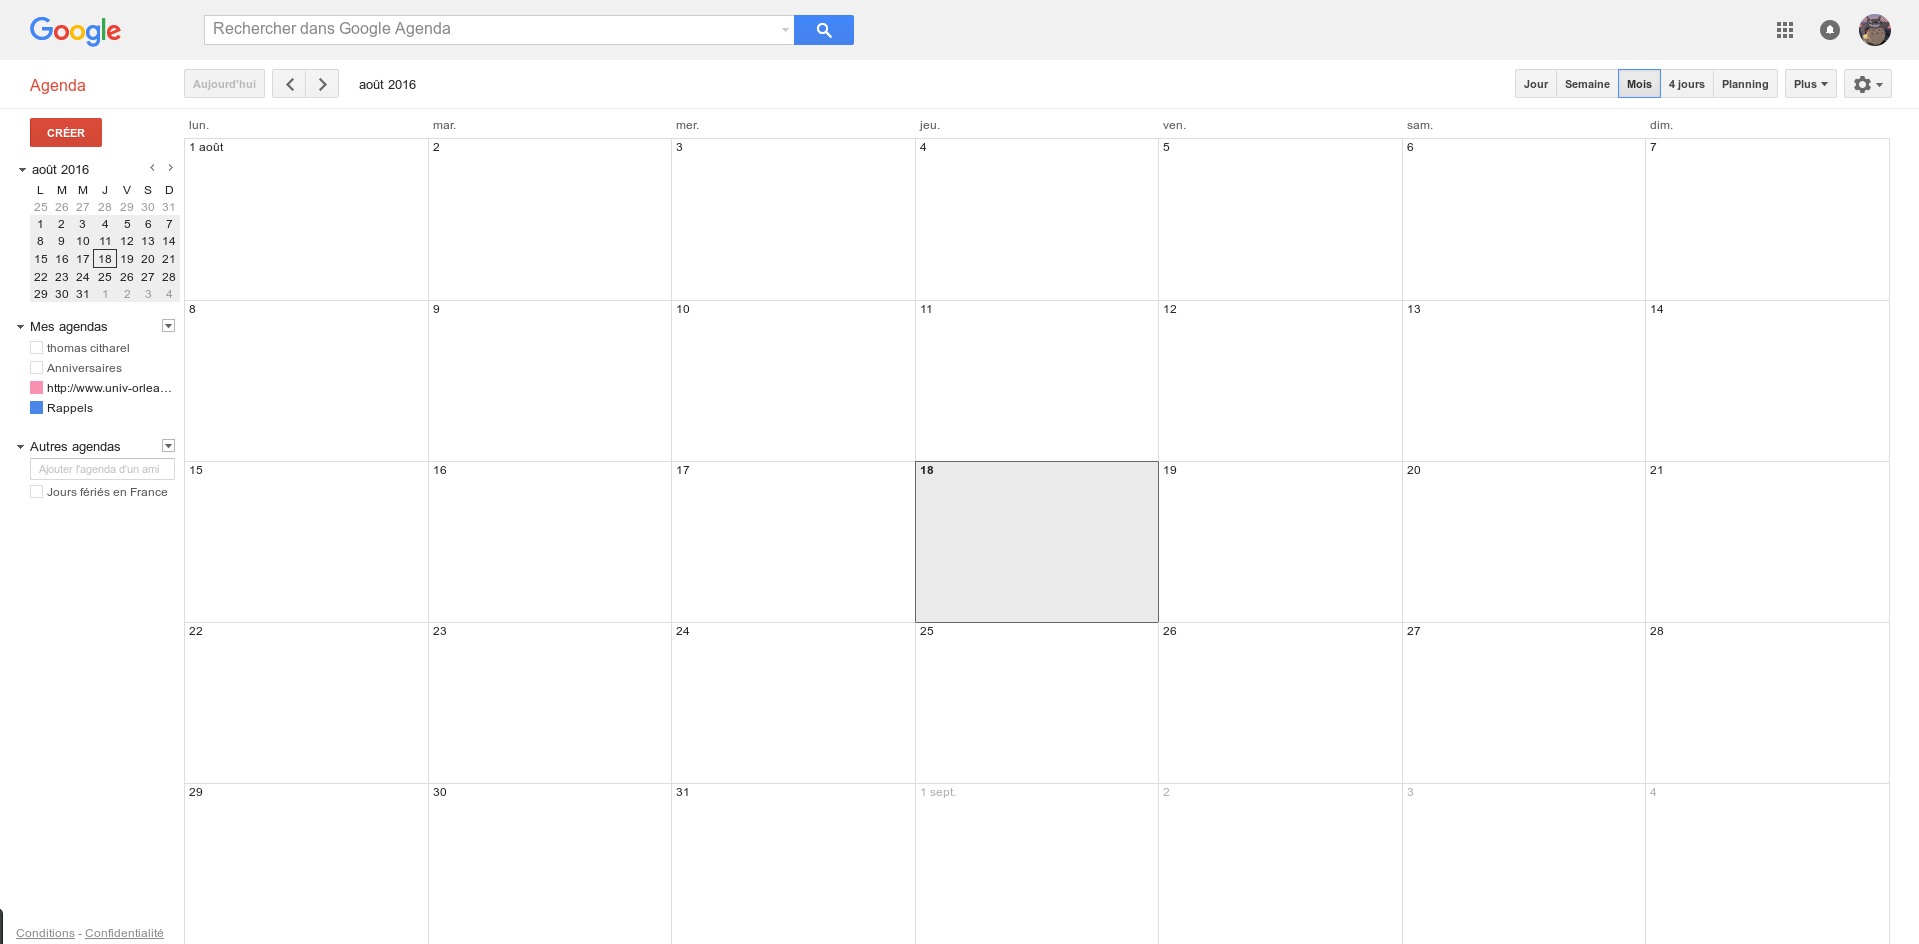
\includegraphics[width=1.5\textwidth]{images/google-agenda-interface-actuelle.png}}
		\caption*{Interface actuelle de Google Agenda}
		\label{normal_case}
	\end{figure}
	
	Ainsi, des applications plus anciennes qui possédaient des fonctionnalités plus avancées ont été écartées car l'interface était non intuitive et la mauvaise qualité du code signifiait apporter une dette technique assez significative.
	
	L'application Calendrier d'ownCloud permettait déjà les fonctionnalités essentielles suivantes.
	
	\subsubsection{Gérer ses calendriers}
	Une des fonctionnalités de base. Lors de la création, on associe un nom et une couleur à un calendrier. Ces propriétés sont éditables et un calendrier peut-être supprimé. On peut afficher les événements associés à un calendrier ou bien les masquer d'un simple clic.
	
	\subsubsection{Gérer des événements}
	Nous pouvons créer des événements, les éditer ou bien les supprimer. Quelques propriétés simples liées à un événement sont ses dates de début et de fin, sa localisation et évidemment sa dénomination. On trouve aussi des fonctionnalités plus avancées, comme pouvoir préciser les participants, définir différentes occurrences de ce même événement, etc.
	
	\subsubsection{Visualisation des événements}
	Les événements sont visibles dans la partie centrale de l'interface. Cette vue peut permettre d'afficher le calendrier sous forme d'un jour ou d'une semaine (comme un agenda), ou bien tout le mois en entier. Un raccourci permet d'accéder directement aux événements pour aujourd’hui.
	
	\subsubsection{Partage de calendriers}
	Un utilisateur peut partager un calendrier (en lecture seule ou en écriture) avec une personne ou un groupe de personnes sur la même instance.
	
	\subsubsection{Import de fichiers calendriers}
	Il est possible d'importer des événements d'un fichier \textit{.ics} dans un des calendriers de l'utilisateur, ou d'en créer un nouveau pour l'occasion.
	
	\subsubsection{Synchronisation avec des clients}
	L'application donne accès aux adresses CalDAV pour synchroniser son calendrier avec un client par exemple sur son téléphone.
	
	\section{Objectifs du stage}
	
	La tâche principale était de sortir un service comme un produit fini, c'est à dire qu'il fallait mettre ajouter les fonctionnalités suivantes, mais également corriger quelques bugs bloquants de manière à ce que le code soit prêt pour l'ouverture du service.
	
	\subsubsection{Permettre de rendre un calendrier public et l'afficher publiquement}
	
	\begin{wrapfigure}{r}{0.4\textwidth}
		\begin{center}
		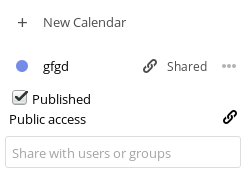
\includegraphics[width=0.3\paperwidth]{images/fonctionnalitepublie.png}
	\end{center}
		\caption{Publication d'un calendrier}
	\end{wrapfigure}
	
	La première tâche est liée premièrement à l'implémentation du protocole de publication d'un calendrier à travers un plugin spécialisé dans le cœur d'ownCloud. D'autre part, il nous faut également une interface utilisateur dans l'application Calendrier qui permette de publier et dé-publier un calendrier. Enfin, il était nécessaire de proposer une vue « publique » accessible à tous sans être enregistré pour les calendriers publiés.

	
	\subsubsection{Permettre d'afficher ce calendrier public sur des pages web externes}La seconde tâche était relativement plus aisée et consistait surtout à configurer l'application correctement pour autoriser l'intégration à l'intérieur de sites tiers, et de rendre son apparence acceptable.
	
	\begin{figure}[ht]
		\centering
		\centerline{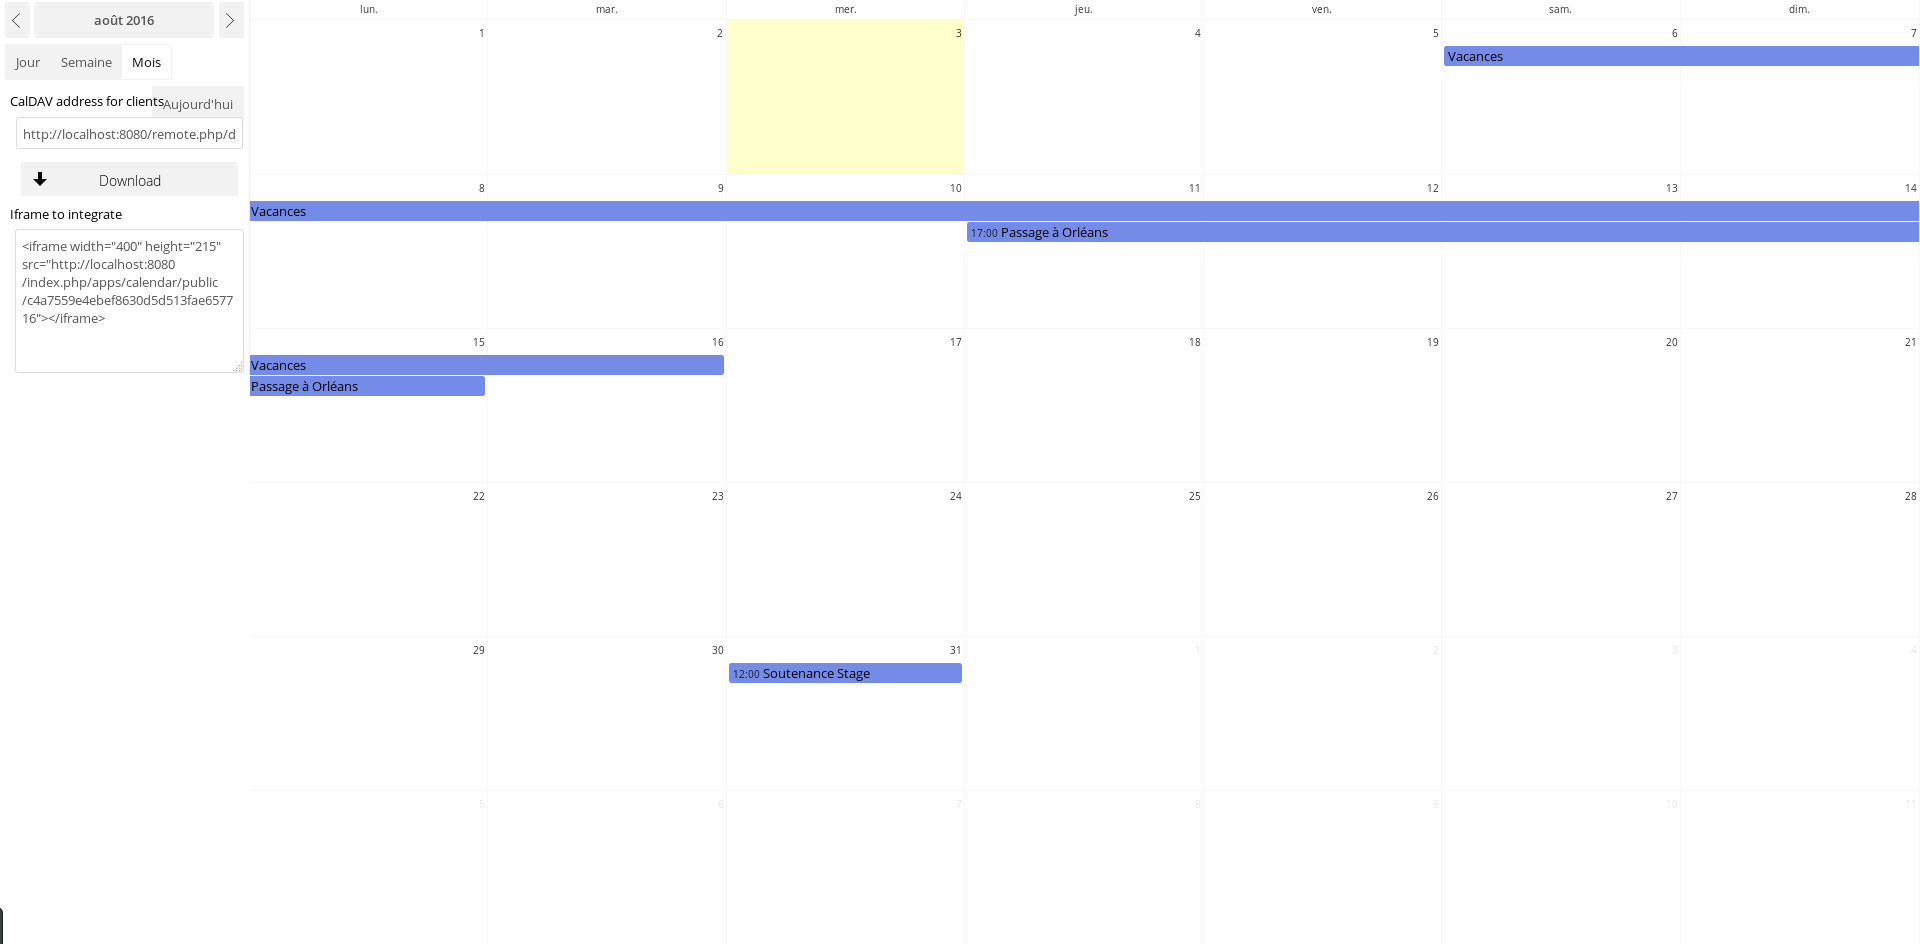
\includegraphics[width=1.5\textwidth]{images/calendrier-vue-publique.png}}
		\caption*{Vue publique d'un calendrier}
		\label{normal_case}
	\end{figure}
	
	%\begin{figure}[ht]
	%	\centerline{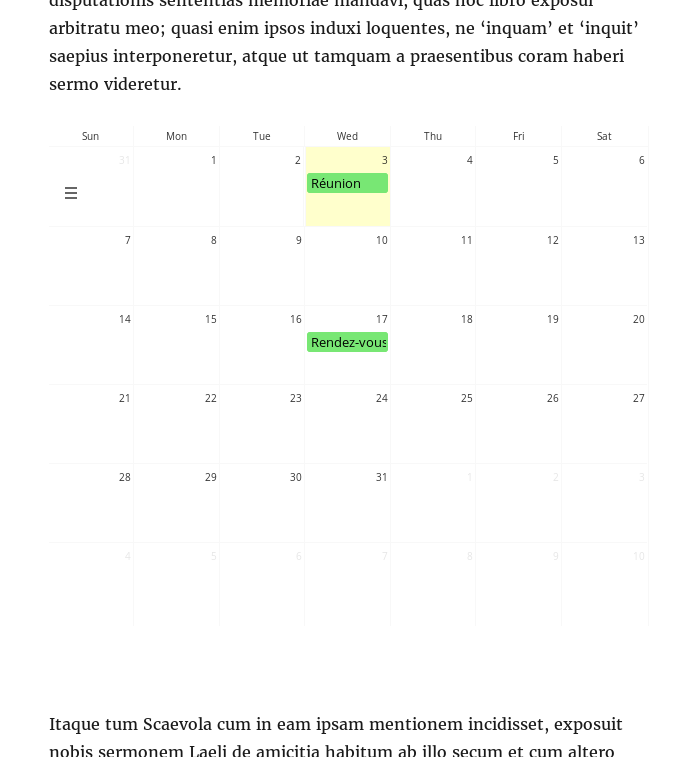
\includegraphics[width=0.65\paperwidth]{images/integration_wordpress}}
	%	\caption*{Intégration d'un calendrier public dans une page Wordpress}
	%	\label{normal_case}
	%\end{figure}
	
	\subsubsection{Permettre de s'abonner à des calendriers}
	
	\textbf{\color{red}NOTE : CHANGER LA CAPTURE D'ÉCRAN}
	\begin{wrapfigure}{r}{0.4\textwidth}
		\begin{center}
			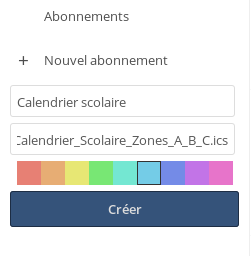
\includegraphics[width=0.40\textwidth]{images/creation_abonnement.png}
		\end{center}
		\caption*{Formulaire pour ajouter un calendrier public}
	\end{wrapfigure}
	
	La troisième tâche consistait à pourvoir une fonctionnalité d'abonnement à des calendriers issus d'une source publique sur internet dans l'application Calendrier d'ownCloud. En effet, l'implémentation des abonnements selon le standard CalDAV était déjà réalisée dans le cœur d'ownCloud, il suffisait de réaliser les bons appels aux API et de gérer les fichiers distants du côté de l'application Calendrier.
	
	\chapter{Analyse de l'existant}
	
	Le fonctionnement des calendriers dans ownCloud est le suivant. Le serveur s'appuie sur la librairie SabreDAV en l'adaptant pour son utilisation particulière dans un module propre. Ce module prend en charge les requêtes suivant le standard CalDAV et sert les données aux clients CalDAV.
	L'application Calendrier fonctionne exactement comme un client CalDAV standard.
	
	\begin{figure}[ht]
		\centering
		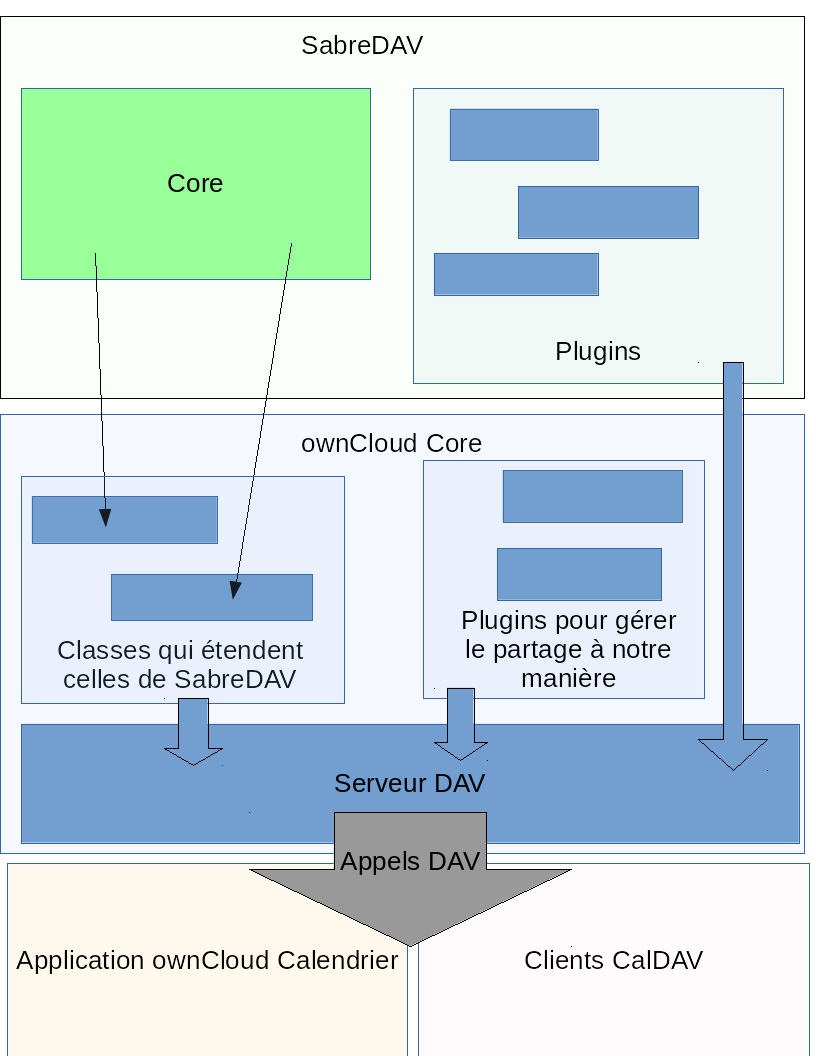
\includegraphics[width=0.75\textwidth]{images/schema.png}
		\caption*{Fonctionnement des calendriers dans ownCloud}
		\label{normal_case}
	\end{figure}
	
	\section{Historic}
	\textbf{\color{red}FAIRE QUELQUE CHOSE AVEC CETTE PARTIE}
	
	
	La première semaine de mon stage a été dédiée à l'étude du fonctionnement du cœur d'ownCloud et de son intégration avec la librairie SabreDAV. J'ai dû également rechercher beaucoup d'informations sur les standards de CalDAV (ainsi que ce qui n'est pas standardisé !) car la synchronisation devait fonctionner à partir des clients existants.
	
	D'autre part, j'ai également dû lire beaucoup du code de l'application Calendrier, car elle est développée à l'aide du Framework AngularJS qui n'est pas exactement une technologie que je maîtrisais.
	
	\section{ownCloud}
	\textbf{ownCloud} est une application web libre écrite dans le langage de programmation PHP. Elle a été initialement créée en 2008 comme une alternative au service Dropbox par Frank Karlitschek. L'application est sous double licence : la licence AGPLv3 et une licence propriétaire qui s'applique à l'édition pour entreprises.
	
	Elle consiste en un cœur (dénommé par la suite comme le \textit{core}) qui s'occupe essentiellement de la gestion des utilisateurs, de la gestion des fichiers, de la gestion des partages et de la fédération et propose des API aux applications tierces afin de faciliter leur intégration. D'autres applications (comme une application de gestion de calendrier, de gestion de contacts, de client de messagerie électronique, de prise de notes ou encore de lecteur de flux RSS) peuvent ainsi intégrées à ownCloud.
	
	\begin{figure}[ht]
		\centering
		
\includegraphics[width=0.5\textwidth]{images/owncloud-logo.png}
		\caption*{Logo ownCloud}
		\label{normal_case}
	\end{figure}
	
	ownCloud peut être installé sur tout hébergement mutualisé qui propose au moins une version de PHP supérieure ou égale à la version 5.4, et propose également des paquets installables automatiquement sur les principales distributions à travers leurs dépôts. De plus, il est proposé à l'administrateur le choix en termes de système de bases de données entre \textit{SQLite}, \textit{MariaDB}/\textit{MySQL} et \textit{PostgreSQL}.
	
	Quelques mois avant que mon stage débute, ownCloud a sorti une version 9 qui a transféré le module DAV (serveur responsable du calendrier et des contacts) dans le \textit{core} et la logique de l'application Calendrier a été refaite complètement quasiment intégralement en JavaScript à l'aide du framework \textit{AngularJS}.
	
	D'autre part, une partie des salariés travaillant ownCloud n'étaient pas satisfaits des décisions de l'entreprise, et ont donc fondé leur propre société. Ils ont effectué un \textit{fork} de l'application sous le nom de NextCloud. Une des différences majeures avec ownCloud est que NextCloud est licenciée uniquement avec la licence AGPL, même pour l'édition Entreprise. Cette scission n'a heureusement pas eu trop de conséquences car il s'est avéré que les deux projets continuaient à communiquer et à échanger du code.
	
	\chapter{Développement}
	\section{Organisation du travail}
	\begin{figure}[ht]
		\centering
		\centerline{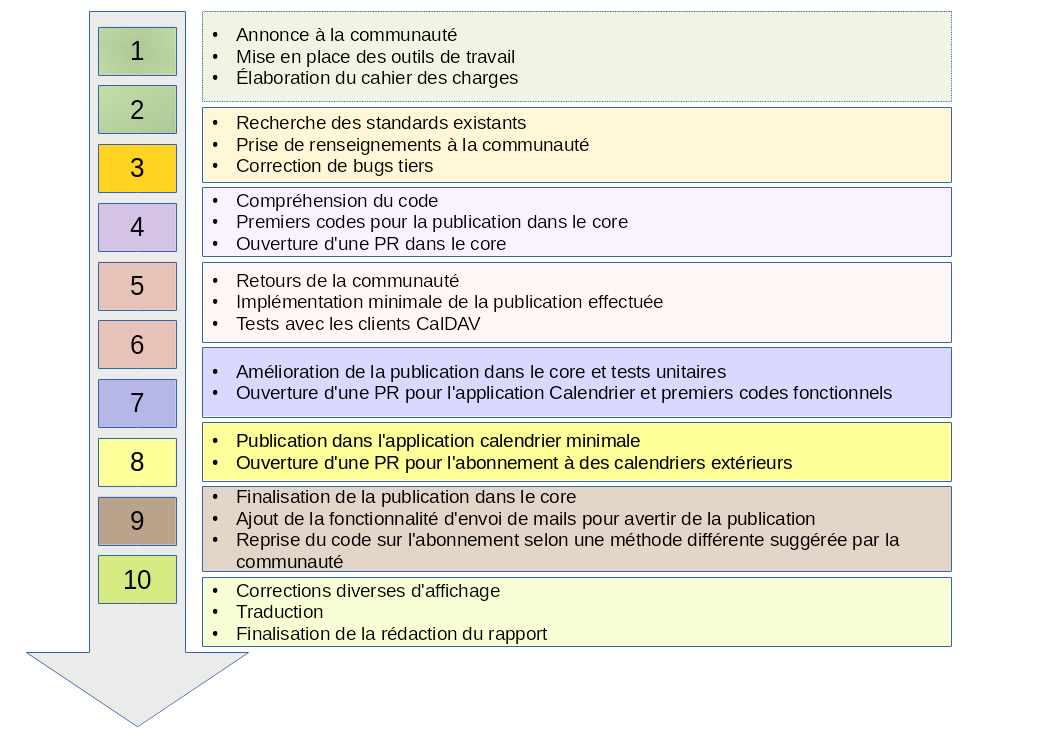
\includegraphics[width=1.45\textwidth]{images/deroulement.png}}
		\caption*{Déroulement du stage}
		\label{normal_case}
	\end{figure}
	
	\section{Environnement technique}
	Mes outils de développement au quotidien se composaient de l'éditeur Atom, de Firefox et de Chromium comme navigateurs. L'application est servie à l'aide du serveur intégré à PHP. Pour le développement, l'application utilisait comme base de données SQLite pour sa simplicité d'utilisation mais lors de changements dans la base de données il a fallu également tester la compatibilité des modifications avec MySQL et PostgreSQL.
	ownCloud utilise git pour la gestion de leur code à travers la forge logicielle Github, qu'ils utilisent également pour le système de tickets. Je me suis donc abonné par courrier électronique à certaines discussions dès le départ afin de suivre certains travaux en cours.
	
	Pour ce qui est de la mise en place de Framagenda, j'ai d'abord eu accès à une machine virtuelle afin d'effectuer des tests ne pouvant être effectués sur ma machine locale, comme l'envoi de courriers électroniques à partir d'un serveur. D'autre part, une instance sur internet m'a aussi permis de demander à des personnes au sein de l'association de faire des tests fonctionnels et d'avoir des premiers retours.
	
	Lors de la mise en production, une machine virtuelle a été dédiée à Framagenda, et l'administrateur système s'est occupé de la configuration de sécurité de base et de la mise en place d'un certificat \textsc{HTTPS} avec le projet \textit{Let's Encrypt}, tandis que j'ai mis en place l'application en elle-même ainsi que configuré proprement le serveur web \textit{nginx} et le serveur de base de données \textit{MariaDB}.
	
	Le code de l'application installé sur les machines provenait directement de mon propre dépôt git sur la forge logicielle proposée par l'association - Framagit - et dont le code correspondait à peu près à celui proposé sur Github, les modifications particulières applicables pour Framagenda en plus. Enfin, là où j'avais une branche pour chaque fonctionnalité dans Github, je m'efforçais d'avoir une branche « produit fini » où les différentes branches étaient fusionnées dans Framagit.
	
	\section{Fonctionnalités}
	\subsection{Publication d'un calendrier}
	Pour pouvoir publier un calendrier il nous fallait donc plusieurs choses : d'abord introduire dans le \textit{core} la gestion de cette propriété, c'est à dire lorsqu'on interroge la ressource calendrier sur ses propriétés, fournir celle-ci en disant le cas échéant si le calendrier est publié.
	Ensuite, il nous fallait introduire un mécanisme pour pouvoir répondre à un appel d'API pour publier ou dépublier le calendrier. Enfin, il fallait que le calendrier publié soit mis dans une collection de ressources à part accessibles à tout le monde.
	
	Je n'ai pas compris cet aspect tout de suite. Je pensais qu'il suffisait de garder la ressource existante et de forcer l'authentification à être désactivée dans ce cas précis.
	
	Tous ces mécanismes ont été réalisés de la même manière (avec les mêmes noms de propriétés) selon laquelle Apple utilise la fonctionnalité de publication dans son application Calendar, et le serveur de Calendrier ownCloud devrait donc être compatible avec ce client.
	
	Il a d'abord fallu changer un peu le \textit{backend}, c'est à dire la manière dont l'application va traiter les données pour les stocker dans la base de donner pour sauvegarder ce nouveau statut du calendrier.
	
	J'ai profité du fait que les partages de calendrier entre utilisateurs étaient stockés dans une table \textit{dav\_shares} où la colonne \textit{access} comprenait un chiffre qui désignait le niveau d'accès au fichier.
	
	J'ai donc rajouté un niveau d'accès qui correspondait à un partage public, ainsi qu'une nouvelle colonne pour stocker l'URL une fois qu'elle serait publiée. 
	
	En effet, l'URL publique se constitue ainsi : 
	\begin{verbatim}
	https://mondomaine.tld/index.php/apps/calendar/public-calendar/<token>
	\end{verbatim}
	qui va chercher les données du calendrier à l'adresse
	\begin{verbatim}
	https://mondomaine.tld/remote.php/public-calendars/<token>
	\end{verbatim}
	
	Comme le token est calculé à partir des informations de base du calendrier (comme son identifiant unique), si je n'avais pas cette colonne supplémentaire pour stocker l'adresse finale de la ressource, il faudrait itérer sur tous les calendriers partagés sur le serveur et vérifier que leur hash correspond bien à celui fourni dans l'URL publique. Alors que dans ce cas je peux savoir directement s'il existe un calendrier pour cette URL publique et le cas échéant récupérer ses informations.
	
	Ensuite, il a fallu écrire un plugin pour SabreDAV pour générer ces propriétés proprement et l'intégrer dans le serveur. Une classe s'occupant de la sérialisation - c'est à dire la conversion des données dans un format texte structuré, ici XML - a également été nécessaire.
	
	On notera que la propriété transmise - l'url du calendrier publié - est connue dès la création du calendrier (car basée sur un \textit{hash} de son identifiant et d'un sel) et est transmise par la propriété \textit{pre-publish-url} avant la publication et ensuite par la propriété \textit{publish-url} dès lors que le calendrier est publié.
	
	Pour prendre en charge la publication et la dépublication, notre plugin a dû intercepter les requêtes POST qui contenaient une propriété particulière.
	En l'occurence, si la requête s'effectuait à l'adresse d'une ressource calendrier et qu'elle contenait l'élément XML \textit{publish-calendar} ou \textit{unpublish-calendar}, nous traitons la requête dans un sens ou dans l'autre et empêchons le traitement de cette dernière par d'autres plugins.
	
	Enfin, pour qu'un calendrier soit disponible publiquement, il a fallu créer un type spécifique de collection de ressources sur lesquelles un utilisateur non-authentifié peut lire les ressources.
	
	De ce côté le serveur \textit{core} était prêt. Dans l'application Calendrier il fallait proposer une extension de l'interface pour permettre à l'utilisateur possédant un calendrier de pouvoir le publier et le dépublier. Ensuite, il fallait fournir à l'utilisateur le lien de l'interface web publique, qui lui fournir également d'autres informations comme les adresses de synchronisation (CalDAV) ou le lien de téléchargement du fichier calendrier \textit{.ics}.
	
	Cette interface web publique devait par nature se passer d'authentification, et également ne pas montrer l'intégration de l'application au système ownCloud, ne montrant que le calendrier et des informations sur celui-ci.
	
	J'ai cherché un moment comment contourner l'intégration à ownCloud avant de me rendre compte à l'aide du code d'autres applications existantes qu'il s'agissait d'un simple paramètre à passer au \textit{template}, hélas non documenté.
	
	Les détails d'un événement qui sont normalement éditables pour le possesseur du calendrier seraient ici uniquement en lecture-seule.
	
	Enfin, une fonctionnalité que j'ai ajoutée plus tard dans le développement est l'envoi de messages électroniques lorsque le calendrier est publié pour notifier des personnes de sa publication.
	
	\subsection{Les abonnements}
	Le standard CalDAV prévoit la possibilité de s'abonner (ou souscrire) à des sources de calendriers externes (publiques sur internet). Cette fonctionnalité était déjà implémentée dans le \textit{core}, mais l'interface de l'application Calendrier ne permettait pas de le faire. 
	
	J'ai donc rajouté cette fonctionnalité en étendant le modèle AngularJS correspondant à un calendrier pour en faire un modèle d'un abonnement, et rajouté dans l'interface une zone pour ajouter une nouvelle souscription. 
	
	Afin de ne pas récuperer à chaque fois le calendrier distant en ligne, un système de proxy met en cache le fichier calendrier distant.
	
	\subsection{Les tests unitaires}
	Les tests unitaires n'étaient pas forcément requis dans le cas de mon développement, mais ils étaient obligatoires dans le cas où je voulais remonter le code \textit{upstream} (en amont) à la communauté. ownCloud, NextCloud et la plupart des applications développent en utilisant la technique d'intégration continue, c'est-à-dire que chaque nouveau morceau de code apporté sur Github lançait l'exécution de la batterie de tests au complet. 
	
	Chaque nouvelle méthode de mon code devait par conséquent s'accompagner d'un test qui devait être préalablement vérifié en local. Si une partie du code que j'avait apportée n'était pas testée, alors le \textit{code coverage}, la proportion de code couvert par les tests par rapport au code complet baissait et cela m'était automatiquement signalé. Les tests unitaires étaient réalisés à l'aide du \textit{framework} de test \textit{PHPUnit} pour le code PHP et de la librairie \textit{Karma} pour le JavaScript de l'application Calendrier.
	
	\subsection{Les trucs annexes}
	
	\textbf{\color{red}TODO : PASSER SUR TOUS LES BUGS CORRIGÉS PAR MOI VOIR SI Y A RIEN À MENTIONNER}
	
	Mon stage consistait avant tout à implémenter de nouvelles fonctionnalités dans l'application Calendrier existante, mais il fallait également que celle-ci soit prête à être utilisée dans Framagenda sans \textit{bugs} flagrants. Ainsi, j'ai corrigé quelques problèmes tiers dans le \textit{core} ou l'application Calendrier.
	On peut citer par exemple les propriétés CalDAV d'un abonnement à un calendrier qui n'étaient pas proprement sauvegardées lors d'une requête de mise à jour ou encore les événements d'un calendrier qui s'effaçaient si jamais l'éditeur était ouvert puis l'action d'édition annulée. 
	
	De plus, afin d'avoir un style de code commun pour tous les contributeurs dans les feuilles de style CSS de l'application Calendrier, j'ai proposé d'utiliser un outil de \textit{lint} CSS et corrigé toutes les feuilles de style en accord. 
	
	Cet outil signale lorsque le code écrit ne suit pas les règles définies, par exemple l'espacement entre les blocs CSS ou l'écriture de règles désuètes.
	
	J'ai aussi ajouté les vérifications faites par cet outil au système d'intégration continue de sorte que si quelqu'un propose une \textit{pull request} qui ne satisfasse pas les règles, elle soit marquée comme erronée.
	
	\mychapter{5}{Bilan du stage}
	\textbf{\color{red}TODO}
	\section{Bilan technique}
	\section{Bilan humain}
	C'était cool.
	\mychapter{6}{Glossaire}
	\begin{itemize}
		\item \textbf{pad} : Éditeur de texte collaboratif en ligne (comme un iPad mais ne fait pas mal). BEST JOKE EVER OMG.
	\end{itemize}
	\mychapter{7}{Abréviations}
	\mychapter{8}{Webographie}
	\mychapter{9}{Annexes}
	\label{ch:Annexes}
	\section{Liste des services de Framasoft}
	\label{sec:listeservices}
	
	\centerline{\begin{tabular}{|c|l|l|l|}%M{1cm}
		\hline
		& \multicolumn{1}{c|}{Service Framasoft} & \multicolumn{1}{c|}{En alternative à} & \multicolumn{1}{c|}{Description}\\
		\hline
		\parbox[t]{3mm}{\multirow{6}{*}{\rotatebox[origin=c]{90}{2013}}} & Framapad & Google Docs & Éditeur collaboratif \\ 
		\cline{2-4} 
		& Framadate & Doodle & Planification de rendez-vous et création de sondages \\ 
		\cline{2-4} 
		& Framacalc & Google Spreadsheet & Tableur collaboratif \\ 
		\cline{2-4}
		& Framanews & Feedly & Lecteur de flux RSS \\ 
		\cline{2-4}
		& Framavectoriel & Pixlr & Création d'images au format SVG \\ 
		\cline{2-4}
		& Framindmap & Bubbl.us & Création de cartes mentales \\ 
		\hline
		\parbox[t]{3mm}{\multirow{3}{*}{\rotatebox[origin=c]{90}{2014}}} & \multicolumn{3}{l|}{Début de la campagne Dégooglisons Internet} \\
		\cline{2-4}
		& Framasphère & Facebook & Réseau social \\ 
		\cline{2-4}
		& Framabag & Pocket & Sauvegarde et lecture différée d'articles\\ 
		\hline
		\parbox[t]{3mm}{\multirow{9}{*}{\rotatebox[origin=c]{90}{2015}}} & Frama.link & bit.ly & Réducteur d'URL \\ 
		\cline{2-4}
		& Framadrive & Dropbox & Sauvegarde de fichiers \\ 
		\cline{2-4}
		& Framagit & Github & Hébergement de code \\ 
		\cline{2-4}
		& Framacarte & Google Maps & Cartographie\\ 
		\cline{2-4}
		& Framabee & Google Search & Moteur de recherche \\ 
		\cline{2-4}
		& Framapic & Imgur & Envoi d'images \\ 
		\cline{2-4}
		& Framabin & Pastebin & Notes anonymes \\
		\cline{2-4}
		& Framaboard & Trello & Gestion de projets \\
		\cline{2-4}
		& Framadrop & Wetransfer & Transfert de fichiers \\
		\hline
		\parbox[t]{3mm}{\multirow{7}{*}{\rotatebox[origin=c]{90}{2016}}} & Framateam & Slack & Communication collaborative \\
		\cline{2-4}
		& Framavox & Shrtct & Prise de décisions \\
		\cline{2-4}
		& \cellcolor{lightgray}Framaforms & \cellcolor{lightgray}Google Forms & \cellcolor{lightgray}Questionnaires en ligne \\
		\cline{2-4}
		& \cellcolor{lightgray}Framapétition & \cellcolor{lightgray}Avaaz & \cellcolor{lightgray}Création de pétitions \\
		\cline{2-4}
		& \cellcolor{lightgray}Framatalk & \cellcolor{lightgray}Skype & \cellcolor{lightgray}Visioconférence \\
		\cline{2-4}
		& \cellcolor{lightgray}Framalistes & \cellcolor{lightgray}Google Groupes & \cellcolor{lightgray}Listes de diffusion \\
		\cline{2-4}
		& \cellcolor{lightgray}Framagenda & \cellcolor{lightgray}Google Agenda & \cellcolor{lightgray}Agenda partagé \\
		\hline 
		\end{tabular}}
	
	Les éléments grisés ne sont pas encore sortis cette année.
	\section{Les standards de gestion de calendrier}
	Un serveur de calendrier doit suivre les standards \textbf{CalDAV}, qui est une extension du protocole \textbf{WebDAV} appliquée aux fichiers \textbf{iCalendar} (\textit{.ics}). WebDAV est un protocole de gestion de fichiers sur serveurs distants conçu comme une extension du standard HTTP. Il a commencé par être standardisé par l'IETF en xxxx.
	
	\href{https://tools.ietf.org/html/rfc2445}{iCalendar}, pour sa part est un standard assez vieux (1998 !) qui décrit le format d'un fichier agenda. Ce format est beaucoup décrié aujourd'hui car étant assez lourd et complexe à manipuler. Heureusement, il existe de nombreuses librairies nous évitant de traiter directement ce format.
	
	Dans notre cas, le serveur est - heureusement - géré avec le concours d'une librairie du nom de \textbf{SabreDAV} qui prend en charge CalDAV, CardDAV (pour les contacts) et WebDAV. Cette librairie fonctionne avec un système de plugins nous permettant de l'adapter pour notre utilisation dans ownCloud.
	
	Il est important de remarquer que si les protocoles et standards internet pour la gestion de calendrier sont définis et correctement documentés, leur implémentations dans les applications clientes ou serveur sont plus qu'hasardeuses et la liste des fonctionnalités supportées peut être assez différente d'une application à l'autre.
	
	Ainsi, c'est la société Apple qui est à la pointe des derniers standards dans son application \textit{iCal} (désormais nommée plus simplement \textit{Calendar}). N'ayant pas de machine Apple, je n'ai pu profiter de ce logiciel pour mes tests.
	
	Le standard WebDAV décrit un protocole pour gérer des ressources - dans notre cas des calendriers - comme un ensemble de méthodes qui étendent celles définies par le standard HTTP. Ces méthodes sont utilisées par des requêtes et des réponses qui structurent les données à l'aide du format XML. Par exemple pour récuperer les propriétés d'une ressource on va utiliser la méthode PROPFIND et si on veut modifier les propriétés d'une ressource la méthode PROPPATCH.
	
	\begin{figure}[ht]
		\centering
		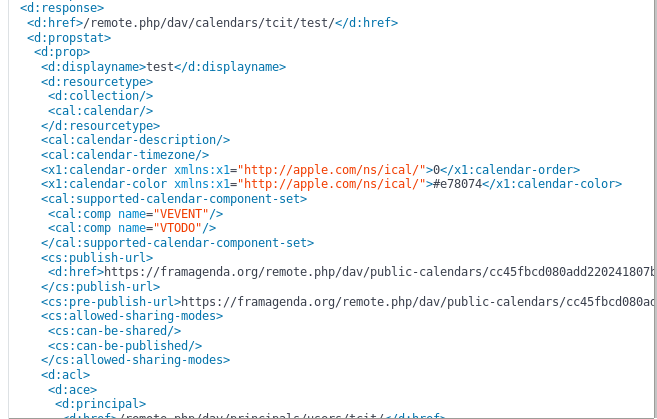
\includegraphics[width=1\textwidth]{images/requete-xml.png}
		\caption*{Extrait d'une requête}
		\label{normal_case}
	\end{figure}
	
	Le standard WebDAV décrit également ce que sont les collections de ressources et comment les droits d'accès (nommés ACL) sont gérés. Par exemple, un utilisateur ne peut accéder qu'à ses fichiers ou à ceux que d'autres utilisateurs ont partagés avec lui.
	
	Le standard XML définit les balises appartenant à un espace de noms. En l'occurence nous avons des balises représentant les propriétés de notre ressource, elle appartiennent ainsi à autant des espaces de noms différents qu'il existe de standards différents qui s'appliquent (IETF, DAV, CalendarServer c'est à dire Apple, et ownCloud pour nos propres propriétés).
	
\end{document}